\chapter{Conception et réalisation de la solution}
\label{chap:trois}

Ce chapitre expose la conception et la réalisation du système. Il présente d'abord le cadre de gestion de projet et la planification, puis l'architecture de la solution, la chaîne de traitement des données, le dispositif d'intelligence artificielle et la modélisation. Il décrit enfin les outils retenus et le protocole de validation et de déploiement.

\section{Méthodologie de gestion de projet et planification}
\label{sec:3-1}

\subsection{Cadre méthodologique retenu}

Le projet associe deux natures de travail que les cadres de référence traitent séparément : la construction d'une application de gestion et la constitution puis l'exploitation d'un gisement de données. Le cadre retenu combine en conséquence deux références.

Le volet données suit le cycle \textbf{CRISP-DM}, dont les six phases --- compréhension du métier, compréhension des données, préparation, modélisation, évaluation, déploiement --- décrivent la progression suivie. Le rapport lui-même en porte la trace : le chapitre~1 traite de la compréhension du métier, le chapitre~2 des données, le présent chapitre de la modélisation et le chapitre~4 de l'évaluation.

Ce cycle a été parcouru plusieurs fois. La phase de compréhension des données a démenti à deux reprises des hypothèses formulées lors de la phase précédente --- le tarif de redevance au mètre carré, puis l'exclusion du sous-sol du parc locatif --- ce qui a imposé de revenir à la compréhension du métier avant de poursuivre. Cette itération n'est pas un accident de parcours mais la propriété que le cadre cherche à produire.

Le volet applicatif suit une démarche \textbf{itérative et incrémentale}, organisée module par module dans l'ordre de leurs dépendances. Chaque module est livré complet --- migrations, modèles, services, écrans, tests --- avant que le suivant ne commence, de sorte qu'à tout instant l'application est dans un état exécutable.

Le pilotage s'appuie sur trois instruments versionnés avec le code, afin qu'aucune décision ne survive hors du dépôt : le dépôt Git, dont chaque message de commit décrit l'intention plutôt que le fichier touché ; un journal de bord consigné chaque soir, qui constitue la matière du présent chapitre et du suivant ; et un registre de dette technique recensant les écarts assumés entre la conception et l'implémentation, qui alimente directement la section~\ref{sec:4-2-3}.

\subsection{Découpage, responsabilités et calendrier}

Le découpage suit l'ordre de dépendance des modules, chaque activité produisant un livrable exécutable et testé. Les durées ont été estimées sur une fenêtre courant du 20~août au 5~septembre~2026, avec une date de gel du code fixée au 3~septembre. Cette date est intangible : les deux derniers jours sont réservés à la rédaction et aux tests, jamais au développement.

Trois règles de conduite encadrent ce planning. Un jour de retard se compense par une coupe de périmètre et non par une extension de la journée de travail, la coupe portant en priorité sur le portail public. Une seule fonctionnalité d'intelligence artificielle est retenue, complète et démontrable, plutôt que plusieurs à moitié faites. Le dépôt est sauvegardé à distance dès le premier jour, avec des envois quotidiens.

Le projet a été conduit par un stagiaire unique, ce qui concentre sur une même personne les rôles de chef de projet, d'analyste, de développeur et de testeur. Cette configuration présente un risque connu, celui de l'absence de relecture par un tiers, traité par deux dispositifs : une suite de tests automatisés servant de relecteur mécanique, et la soumission des arbitrages métier à la coordination du Village. L'encadrement académique a assuré la supervision méthodologique, l'encadrement professionnel l'accès au terrain et la validation des besoins, et la coordination du Village l'arbitrage des règles de gestion.

\begin{table}[H]
\centering
\caption{Découpage du projet en activités}
\label{tab:wbs}
\singlespacing
\begin{tabularx}{\textwidth}{@{}p{1.1cm}Xp{2.1cm}@{}}
\toprule
\entete{Réf.} & \entete{Activité} & \entete{Durée (jours)}\\
\midrule
A & Collecte de terrain, transcription du registre, mise en place de l'environnement & 4\\
B & Module Socle : village, exercice, utilisateurs, rôles, permissions, journal d'audit & 3\\
C & Module Artisanat : artisans, corps de métier, contenants, espaces locatifs, attributions & 3\\
D & Module Commerce : catégories, produits, dépôts, journal de stock & 3\\
E & Module Commerce : écran de vente, commission, figement & 2\\
F & Module Trésorerie : caisses, sections, brouillard, arrêté journalier & 3\\
G & Module Trésorerie : comptes artisans, campagnes de reversement & 2\\
H & Reprise des données réelles et rapport d'import & 2\\
I & Module Pilotage : tableau de bord et indicateurs & 2\\
J & Module Pilotage : indexation, assistant, protocole d'évaluation & 4\\
K & Module Portail : catalogue public, fiches artisans, contenus éditoriaux & 3\\
L & Consolidation, gel du code, rédaction et manuel utilisateur & 4\\
\bottomrule
\end{tabularx}
\onehalfspacing
\source{élaboré par l'auteur.}
\end{table}

\begin{figure}[H]
\centering
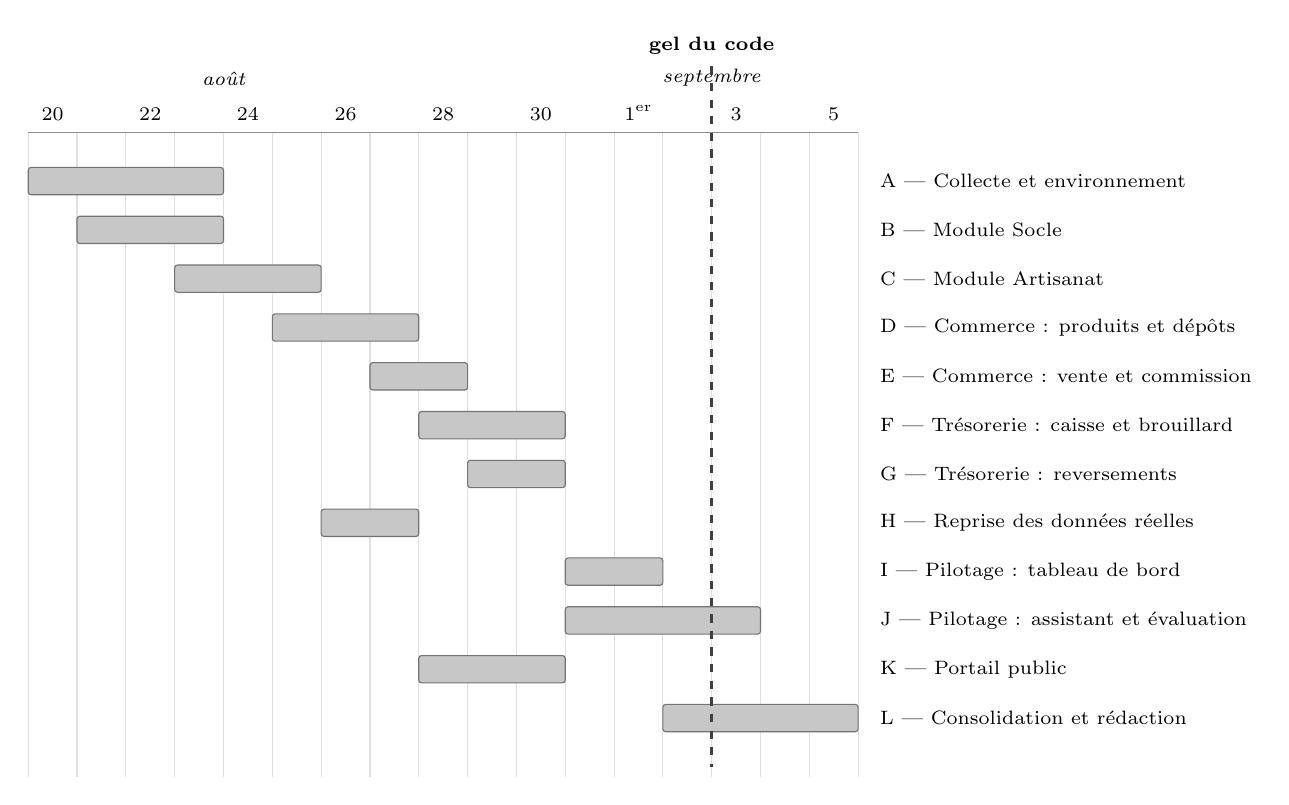
\begin{tikzpicture}[font=\scriptsize,x=0.62cm,y=0.62cm]
\def\jours{17}
\foreach \i in {0,...,\jours}{\draw[black!12] (\i,0) -- (\i,-13.2);}
\foreach \i/\l in {0/20,2/22,4/24,6/26,8/28,10/30,12/1\textsuperscript{er},14/3,16/5}{
  \node[anchor=south,font=\scriptsize] at (\i+0.5,0.05) {\l};}
\node[anchor=south,font=\scriptsize\itshape] at (4,0.75) {août};
\node[anchor=south,font=\scriptsize\itshape] at (14,0.75) {septembre};
\draw[black!45] (0,0) -- (\jours,0);
\foreach \y/\d/\w/\lab in {%
 1/0/4/{A --- Collecte et environnement},
 2/1/3/{B --- Module Socle},
 3/3/3/{C --- Module Artisanat},
 4/5/3/{D --- Commerce : produits et dépôts},
 5/7/2/{E --- Commerce : vente et commission},
 6/8/3/{F --- Trésorerie : caisse et brouillard},
 7/9/2/{G --- Trésorerie : reversements},
 8/6/2/{H --- Reprise des données réelles},
 9/11/2/{I --- Pilotage : tableau de bord},
 10/11/4/{J --- Pilotage : assistant et évaluation},
 11/8/3/{K --- Portail public},
 12/13/4/{L --- Consolidation et rédaction}}{
  \fill[black!22,draw=black!55,rounded corners=1pt] (\d,-\y+0.28) rectangle (\d+\w,-\y-0.28);
  \node[anchor=west,font=\scriptsize] at (\jours+0.25,-\y) {\lab};}
\draw[very thick,black!75,dashed] (14,1.35) -- (14,-13);
\node[anchor=south,font=\scriptsize\bfseries] at (14,1.4) {gel du code};
\end{tikzpicture}
\caption{Diagramme de Gantt du projet}
\source{élaboré par l'auteur.}
\end{figure}

\section{Architecture, pipeline de données et modélisation}
\label{sec:3-3}

\subsection{Architecture globale de la solution}

La solution est une application web modulaire de près de 37~500~lignes, organisée en six modules dont les dépendances sont strictement descendantes. Un module ne référence que les modules dont il dépend ; aucune dépendance montante n'est autorisée.

\begin{table}[H]
\centering
\caption{Modules de la solution, entités principales et volume}
\label{tab:modules}
\singlespacing
\begin{tabularx}{\textwidth}{@{}p{1.9cm}Xp{1.3cm}@{}}
\toprule
\entete{Module} & \entete{Entités principales} & \entete{Fichiers}\\
\midrule
1. Socle & Village, Exercice, Utilisateur, Agent, JournalAudit, registre de verrous de clôture & 35\\
2. Artisanat & Artisan, CorpsMetier, Entreprise, Boutique, EspaceLocatif, AttributionEspace & 54\\
3. Commerce & CategorieProduit, Produit, Depot, MouvementStock, Vente, LigneVente, TauxCommission & 63\\
4. Trésorerie & Caisse, SectionCaisse, MouvementCaisse, ArreteCaisse, CampagneReversement, Reversement & 75\\
5. Pilotage & FicheLexicale, TermeLexical, TermeVocabulaire ; tableaux de bord et assistant & 77\\
6. Portail & PublicationProduit, ArtisanVedette, ContenuPage, DemandeContact & 44\\
\bottomrule
\end{tabularx}
\onehalfspacing
\source{relevé sur le dépôt du projet ; 34 tables au total.}
\end{table}

Le franchissement d'une frontière obéit à une règle unique : le module \emph{consommateur} déclare l'interface dont il a besoin, et le module \emph{fournisseur} l'implémente et l'enregistre depuis son propre fournisseur de services. Quatre interfaces sont en service. Le Commerce déclare un journal de caisse que la Trésorerie implémente : il peut donc faire écrire une vente en caisse sans jamais connaître la Trésorerie. Le Socle déclare un verrou de clôture auquel la Trésorerie vient se déclarer : un exercice ne peut être clôturé s'il reste une section de caisse ouverte ou une campagne non validée, sans que le Socle ait à connaître ces notions. Il en découle qu'un module peut être retiré sans casser ceux qui le précèdent : le Pilotage et le Portail sont désactivables sans que la chaîne de gestion en soit affectée.

\begin{figure}[H]
\centering
\begin{tikzpicture}[
  font=\footnotesize,
  mod/.style={draw,rounded corners=2pt,align=center,text width=3.4cm,minimum height=9mm,fill=black!5},
  fl/.style={-{Latex[length=2mm]},thick},
  port/.style={-{Latex[length=1.8mm]},dashed,black!60}]

\node[mod,fill=black!12] (socle) {\textbf{1. Socle}};
\node[mod,below=6mm of socle] (art) {\textbf{2. Artisanat}};
\node[mod,below=6mm of art] (com) {\textbf{3. Commerce}};
\node[mod,below=6mm of com] (tre) {\textbf{4. Trésorerie}};
\node[mod,below=6mm of tre] (pil) {\textbf{5. Pilotage}};
\node[mod,below=6mm of pil] (por) {\textbf{6. Portail}};

\draw[fl] (art) -- (socle);
\draw[fl] (com) -- (art);
\draw[fl] (tre) -- (com);
\draw[fl] (pil) -- (tre);
\draw[fl] (por) -- (pil);

\node[align=left,anchor=west,text width=6.2cm,font=\scriptsize] at ($(socle.east)+(1.4cm,0)$)
  {\textbf{Interfaces de franchissement}\\[2pt]
   \textit{VerrouDeCloture} --- déclarée par le Socle,\\ implémentée par la Trésorerie\\[3pt]
   \textit{JournalDeCaisse} --- déclarée par le Commerce,\\ implémentée par la Trésorerie\\[3pt]
   \textit{ModeleDeLangage} et \textit{FournisseurDEmbeddings}\\ --- déclarées par le Pilotage, implémentées\\ par des adaptateurs remplaçables};

\draw[port] ($(socle.east)+(0.15cm,0.2cm)$) -- ++(1.1cm,0);
\draw[port] ($(tre.east)+(0.15cm,0)$) to[bend right=18] ($(socle.east)+(1.25cm,-0.2cm)$);
\end{tikzpicture}
\caption{Architecture modulaire et sens des dépendances}
\source{élaboré par l'auteur.}
\end{figure}

\subsection{Préparation et prétraitement des données}

La constitution du gisement exploitable a représenté une part substantielle du travail. Elle procède en cinq étapes, présentées à la figure~\ref{fig:pipeline}.

La \textbf{transcription} reporte le registre manuscrit en format tabulaire, page par page, en conservant la valeur telle qu'elle est écrite, y compris lorsqu'elle paraît fautive : corriger à la saisie ferait disparaître l'anomalie que l'étude cherche à mesurer. La \textbf{normalisation} ramène ensuite les libellés à une forme canonique --- suppression des accents et de la casse pour les clés de rapprochement, unification des séparateurs, format de date unique --- et distingue les lignes de données des lignes de sous-total que le support mêle dans la même colonne.

La \textbf{déduction contrôlée} reconstitue la troisième valeur lorsque deux des trois --- quantité, prix unitaire, montant --- sont présentes, et rejette la ligne lorsqu'une seule l'est. Cette règle a conduit à reconstituer 602~lignes et à en rejeter une. Chaque déduction est enregistrée comme une anomalie dans le rapport d'import, de sorte que le lecteur sait exactement ce qui a été lu et ce qui a été calculé.

La \textbf{résolution d'entités} compare les écritures de nom du registre aux occupants du relevé par une mesure de similarité de chaînes : au-dessus d'un seuil de 85~\%, le rapprochement est automatique ; en dessous, il est écarté. Le choix d'un seuil élevé produit délibérément des faux négatifs, et ce déséquilibre est voulu. Rapprocher à tort deux artisans revient à attribuer à l'un les ventes de l'autre, donc à fausser un solde dû ; laisser deux écritures distinctes alors qu'elles désignent la même personne produit un doublon visible, qu'un agent corrigera. Le coût des deux erreurs n'est pas symétrique, et le seuil est réglé du côté où l'erreur se voit. Une vérification indépendante du rapprochement, conduite lors de la rédaction, l'a confirmé : un rapprochement plus permissif acceptait \guillemotleft~Ngassam Olivier~\guillemotright{} comme désignant une occupante nommée \guillemotleft~NGASSAM Bernadette~\guillemotright, sur le seul patronyme. Le seuil retenu refuse ce rapprochement, et il a raison.

Le \textbf{rattachement et signalement}, enfin, conserve les lignes dépourvues de correspondance avec le nom porté au registre, sans leur inventer d'espace. Un rapport d'import récapitule l'ensemble des traitements, ligne par ligne et en synthèse ; c'est ce rapport qui fournit les chiffres du tableau~\ref{tab:qualite}.

\begin{figure}[H]
\centering
\resizebox{\textwidth}{!}{%
\begin{tikzpicture}[
  font=\footnotesize,
  src/.style={draw,align=center,text width=2.2cm,minimum height=10mm,fill=black!10},
  et/.style={draw,rounded corners=2pt,align=center,text width=2.3cm,minimum height=10mm,fill=black!4},
  sortie/.style={draw,rounded corners=2pt,align=center,text width=2.4cm,minimum height=10mm,fill=black!12},
  fl/.style={-{Latex[length=2mm]},thick}]

\node[src] (r1) {Registre\\manuscrit};
\node[src,below=4mm of r1] (r2) {Relevé des\\occupants};
\node[src,below=4mm of r2] (r3) {Inventaire\\des produits};

\node[et,right=9mm of r2] (tr) {Transcription\\et normalisation};
\node[et,right=8mm of tr] (dd) {Déduction\\contrôlée};
\node[et,right=8mm of dd] (re) {Résolution\\d'entités};
\node[sortie,right=8mm of re] (bd) {Base\\structurée};

\node[sortie,above right=6mm and 8mm of bd,text width=2.6cm] (ind) {Indicateurs\\{\scriptsize agrégations SQL}};
\node[sortie,below right=6mm and 8mm of bd,text width=2.6cm] (idx) {Index lexical\\{\scriptsize fiches pondérées}};
\node[et,below=5mm of dd,text width=3.4cm,fill=white,draw=black!45] (rap) {Rapport d'import\\{\scriptsize 603 lignes, anomalie par anomalie}};

\draw[fl] (r1) -- (tr); \draw[fl] (r2) -- (tr); \draw[fl] (r3) -- (tr);
\draw[fl] (tr) -- (dd); \draw[fl] (dd) -- (re); \draw[fl] (re) -- (bd);
\draw[fl] (bd) |- (ind); \draw[fl] (bd) |- (idx);
\draw[fl,dashed,black!60] (dd) -- (rap);
\draw[fl,dashed,black!60] (re) |- (rap);
\end{tikzpicture}}
\caption{Chaîne de préparation des données, de la source manuscrite aux deux usages}
\label{fig:pipeline}
\source{élaboré par l'auteur.}
\end{figure}

\subsection{Conception du dispositif d'intelligence artificielle}

\subsubsection{Le partage de responsabilité}

Le dispositif retenu est un assistant d'interrogation en langage naturel. Sa conception repose sur une décision unique, prise avant toute considération technique : \textbf{une question d'agrégation et une question descriptive ne sont pas traitées par le même mécanisme, et les deux mécanismes ne communiquent pas}.

Un routeur classe la question à l'entrée. S'il reconnaît une intention d'agrégation --- chiffre d'affaires, recettes de commission, nombre de ventes, solde dû --- la question part vers un service de rapport qui la résout par une requête d'agrégation, avec des paramètres extraits de la question mais jamais une requête fabriquée à partir d'elle. Sinon, la question part vers la recherche documentaire, qui n'a accès à aucun indicateur.

Il n'existe aucun repli d'une branche vers l'autre. Une question d'agrégation dont le calcul rend zéro reste sur le calcul : autoriser la bascule ferait qu'un chiffre d'affaires nul se transformerait en extraits de fiches produit, qu'un lecteur pressé lirait comme une réponse à sa question financière. Symétriquement, une question descriptive ne remonte jamais vers le service de rapport, faute de quoi la garantie centrale n'en serait plus une.

\subsubsection{Le catalogue d'intentions plutôt que la génération de requêtes}

La solution la plus répandue pour interroger une base en langage naturel consiste à faire produire une requête SQL par un modèle de langage. Elle a été écartée, et le motif tient à la nature des données : le système suit de l'argent public. Une requête fabriquée à partir d'une question mal comprise peut lire ce qu'elle veut ; une intention reconnue dans un catalogue fermé ne peut, au pire, que retourner le mauvais indicateur.

Le score minimal de reconnaissance est fixé à deux termes, et cette asymétrie est voulue. Une expression d'un seul mot --- \guillemotleft~artisans~\guillemotright, \guillemotleft~ventes~\guillemotright{} --- capterait des questions descriptives et les enverrait au calcul. Exiger deux termes renvoie les cas douteux vers la branche descriptive, où ils n'obtiendront rien plutôt qu'un chiffre faux. Un faux négatif coûte une question sans réponse ; un faux positif coûte un montant erroné présenté comme exact.

\subsubsection{Les trois garde-fous}

Trois dispositifs encadrent la branche descriptive.

Le premier est un \textbf{seuil de similarité} en deçà duquel aucune source n'est retenue. Une question sans réponse dans le corpus reçoit un refus explicite, et non les cinq documents les moins mauvais.

Le deuxième est un \textbf{contrôle des chiffres}. Le texte produit est relu avant affichage, et toute suite de chiffres absente des extraits retrouvés provoque un refus. Ce contrôle transforme une discipline en propriété testable : en théorie, une réponse composée uniquement d'extraits ne peut pas inventer de nombre ; en pratique, une phrase de liaison telle que \guillemotleft~trois fiches correspondent~\guillemotright{} en introduit un que personne ne remarque avant la soutenance.

Le troisième est l'\textbf{affichage systématique des sources}. Chaque réponse descriptive est accompagnée des extraits qui l'ont fondée, ce qui permet au lecteur de vérifier plutôt que de croire.

\subsubsection{La rédaction générative et son repli}

Un modèle de langage intervient en aval de la recherche, pour mettre en français suivi les extraits déjà retrouvés. Le port qui l'expose n'offre qu'une seule opération : rédiger à partir d'extraits fournis. Le modèle ne cherche rien, ne calcule rien et ne voit aucun indicateur --- non parce qu'une consigne le lui interdit, mais parce qu'il n'a accès à rien d'où un chiffre pourrait venir.

Deux profils sont configurés, un service local et un service distant, dans cet ordre. Le local passe devant, et le motif n'est pas la qualité : un modèle installé sur la machine ne coûte rien, ne demande aucune clé et ne dépend d'aucune connexion. Il fonctionne donc dans une salle sans réseau, ce qui est la condition de démonstration retenue.

Sans clé, sans modèle et sans réseau, le composant de rédaction rend une valeur nulle et l'assistant liste les extraits. Ce chemin dégradé n'est pas un secours écrit à part : c'est le comportement nominal du premier jour, qui n'a pas été retiré, et il est parcouru par l'intégralité de la suite de tests --- donc mieux éprouvé que le chemin nominal actuel.

\begin{figure}[H]
\centering
\resizebox{\textwidth}{!}{%
\begin{tikzpicture}[
  font=\footnotesize,
  n/.style={draw,rounded corners=2pt,align=center,text width=2.5cm,minimum height=10mm,fill=black!5},
  g/.style={draw,rounded corners=2pt,align=center,text width=2.3cm,minimum height=9mm,fill=black!12},
  fl/.style={-{Latex[length=2mm]},thick}]

\node[n,fill=black!14] (q) {Question en\\langage naturel};
\node[n,right=8mm of q] (rt) {Routeur\\{\scriptsize catalogue d'intentions}};

\node[n,above right=8mm and 9mm of rt,text width=2.7cm] (calc) {Service de rapport\\{\scriptsize agrégation SQL}};
\node[n,below right=8mm and 9mm of rt,text width=2.7cm] (rech) {Recherche lexicale\\{\scriptsize index pondéré}};

\node[g,right=9mm of calc] (mont) {Montant exact};
\node[n,right=9mm of rech,text width=2.6cm] (red) {Rédaction\\{\scriptsize modèle de langage}};
\node[g,right=9mm of red] (rep) {Réponse\\+ sources};

\draw[fl] (q) -- (rt);
\draw[fl] (rt) |- (calc) node[pos=0.72,above,font=\scriptsize\itshape]{agrégation};
\draw[fl] (rt) |- (rech) node[pos=0.72,below,font=\scriptsize\itshape]{descriptive};
\draw[fl] (calc) -- (mont);
\draw[fl] (rech) -- (red);
\draw[fl] (red) -- (rep);
\draw[fl,dashed,black!55] (rech.south) to[bend right=20] node[midway,below,font=\scriptsize\itshape,yshift=-1mm]{repli sans modèle : liste des extraits} (rep.south);

\begin{scope}[on background layer]
\draw[dashed,black!60] ($(rt.east)+(4mm,16mm)$) -- ($(rt.east)+(4mm,-16mm)$);
\end{scope}
\node[font=\scriptsize\bfseries,black!70,anchor=south,rotate=90] at ($(rt.east)+(3mm,4mm)$) {frontière};
\end{tikzpicture}}
\caption{Architecture de l'assistant : deux branches séparées par une frontière infranchissable}
\label{fig:assistant}
\source{élaboré par l'auteur.}
\end{figure}

\subsection{Modèle de données}
\label{sec:3-3-4}

\subsubsection{Le modèle opérationnel}

Le modèle relationnel compte trente-quatre tables réparties sur les six modules. Trois choix de modélisation méritent d'être exposés, car ils découlent directement des constats du chapitre~2.

\textbf{L'espace locatif, et non la boutique, porte la location.} Le contenant est un objet physique ; ce qui se loue est l'espace qu'il abrite. L'attribution, la redevance et la règle de non-chevauchement portent donc sur l'espace. Le modèle initial attribuait la boutique : il refusait la cohabitation, qui est la situation ordinaire, et ne protégeait pas le partage d'un même espace, qui est la vraie faute. La table des contenants porte en outre une colonne de nature --- boutique, sous-sol, espace vert --- afin que le taux d'occupation présenté à la tutelle reste calculable sur les seuls locaux de vente.

\textbf{La vente fige ses valeurs.} À l'enregistrement, une vente recopie la référence et la désignation du produit, le prix unitaire, la quantité, l'espace, l'artisan et le taux de commission. Ces valeurs ne sont jamais recalculées depuis les référentiels. Sans ce figement, la modification ultérieure d'un prix réécrirait rétroactivement l'histoire commerciale du village.

\textbf{Les soldes sont calculés, jamais stockés.} Le solde dû à un artisan est la différence entre la somme de ses parts et la somme de ses reversements. La quantité en stock d'un produit est le solde de ses mouvements. Un champ modifiable porterait une valeur qui, un jour, ne correspondrait plus à ses composantes, sans que rien ne le signale.

\subsubsection{Le modèle dimensionnel}

Sur ce modèle opérationnel se greffe une lecture analytique en étoile, dont le grain est la ligne de vente et les dimensions l'artisan, le produit, l'espace locatif, le vendeur et le temps. Cette organisation n'est pas matérialisée dans une base distincte --- la volumétrie ne le justifie pas --- mais elle structure les requêtes d'agrégation du tableau de bord et les intentions reconnues par l'assistant.

\subsubsection{Une limite du modèle des prix, contenue et non corrigée}

Le chapitre~2 a établi qu'un même produit peut exister sous plusieurs conditionnements à des prix distincts. Le modèle retenu ne le représente pas : le prix unitaire est un montant unique porté par le produit, et un produit à deux conditionnements se modélise par deux produits.

Ce défaut n'est pas né du modèle, il y est devenu visible. Le registre le portait déjà, caché dans la désignation. Le corriger supposerait de rouvrir la règle de figement, l'écran de vente, la procédure d'import et les six cents ventes déjà chargées.

Le choix retenu est de contenir le défaut plutôt que de le masquer. Lorsqu'une fiche technique de produit porte plusieurs montants, le système les repère, les compte et n'en reporte aucun dans le formulaire : un prix pré-rempli serait faux deux fois sur trois, et faux en silence. Un signalement explicite prévient l'agent, qui saisit le prix du produit effectivement enregistré. La représentation d'un produit porteur de plusieurs conditionnements est renvoyée à une version ultérieure.

\subsection{Modèle de rôles et d'habilitations}

Les rôles applicatifs calquent l'organigramme présenté au chapitre~1 : coordonnateur, coordonnateur adjoint et cinq chefs de section. Les permissions sont nommées selon le motif \emph{action\_entité} et vérifiées à l'affichage de chaque action. Deux principes structurent ce modèle.

Le premier est que \textbf{le coordonnateur n'est pas le super-utilisateur}. Le coordonnateur est un rôle métier adossé à une fonction ; le super-utilisateur est un compte technique qui peut tout, y compris s'attribuer des droits et administrer les rôles. Les fusionner permettrait à une personne exerçant une fonction administrative de modifier ses propres permissions et d'effacer des traces --- exactement ce qu'un contrôle interne cherche à empêcher dans une structure qui manipule de l'argent public. En exploitation, le coordonnateur du village portera probablement les deux rôles ; ce sera une décision d'attribution explicite, jamais une propriété du modèle de données.

Le second est la \textbf{séparation des fonctions selon la nature du risque}. Une responsabilité qualitative --- valider un produit --- peut être suppléée par la hiérarchie, faute de quoi l'absence d'une seule personne bloque le flux principal ; le journal d'audit conserve alors l'identité du validateur réel. Une responsabilité financière --- clôturer une section de caisse, valider une campagne de reversement --- ne se supplée pas, parce que le risque n'y est pas l'immobilisme mais l'auto-attribution d'un avantage.

Il en découle une règle appliquée partout : \textbf{une trace se constate, elle ne se choisit pas}. Un champ qui enregistre \emph{qui} a fait quelque chose prend le compte connecté, jamais une valeur choisie dans une liste. Si la mauvaise personne peut agir, la réponse est de lui retirer la permission, non d'ouvrir une liste déroulante.

\section{Outils, validation et déploiement}
\label{sec:3-4}

\subsection{Choix technologiques}

\begin{table}[H]
\centering
\caption{Choix technologiques et justification}
\label{tab:techno}
\singlespacing
\begin{tabularx}{\textwidth}{@{}p{3.2cm}p{2.2cm}X@{}}
\toprule
\entete{Composant} & \entete{Technologie} & \entete{Motif du choix}\\
\midrule
Langage serveur & PHP 8.3 & Disponible sur tout hébergement mutualisé ; coût de mise en service nul\\
Cadriciel applicatif & Laravel 12 & Persistance, migrations, événements, conteneur d'injection\\
Interface d'administration & Filament 5 & Écrans générés depuis les modèles, en français\\
Découpage modulaire & \emph{laravel-modules} & Frontières de module matérialisées dans l'arborescence\\
Rôles et permissions & \emph{laravel-permission} & Modèle de rôles standard, éprouvé\\
Base de données & PostgreSQL 14 & Contraintes d'intégrité, agrégations performantes\\
Documents imprimables & \emph{laravel-dompdf} & Reçus, décharges, états de reversement\\
Vectorisation (mesure) & Ollama & Exécution locale, sans coût ni clé\\
Rédaction générative & Interface compatible & Fournisseur interchangeable par configuration\\
Modélisation & UML & Cas d'utilisation, classes, séquences\\
\bottomrule
\end{tabularx}
\onehalfspacing
\source{élaboré par l'auteur.}
\end{table}

Le choix de PHP et de Laravel plutôt que d'une pile plus récente répond directement au risque identifié au chapitre~1 : un projet antérieur de la structure est resté non déployé faute de budget d'hébergement. Une application PHP fonctionne sur l'hébergement mutualisé le moins coûteux du marché, et sur un simple poste du village en réseau local. Ce critère a primé sur toute considération de modernité.

Deux difficultés propres à l'environnement de développement méritent d'être consignées, car elles se reproduiront lors du déploiement sur le poste du village. PHP sous Windows n'embarque aucun magasin de certificats racine, de sorte que tout appel sortant en HTTPS échoue tant que les chemins de certificats ne sont pas déclarés dans sa configuration. Le correctif le plus fréquemment proposé --- désactiver la vérification du certificat --- a été écarté : dans un système qui manipule de l'argent public, retirer délibérément l'authentification du serveur distant est indéfendable. L'échec correspondant était en outre silencieux pour l'utilisateur, le repli le rattrapant ; il a fallu ajouter une trace explicite dans les journaux pour qu'il devienne visible au développeur.

\subsection{Protocole de validation}

La validation repose sur une suite de tests automatisés qui couvre les règles de gestion, les habilitations et les conventions d'écriture. Les \textbf{tests de règle métier} éprouvent le comportement observable attendu : qu'une vente fige ses valeurs, qu'un mouvement de caisse refuse d'être modifié, qu'un exercice ne se clôture pas si une section reste ouverte, qu'un solde d'artisan se recalcule depuis ses composantes. Les \textbf{tests d'habilitation} éprouvent l'accès en exécution avec un compte non privilégié, y compris par accès forgé à une action que l'interface n'affiche pas. Un \textbf{test de conventions} parcourt statiquement l'ensemble des écrans de tous les modules et échoue si une action est déclarée sans contrôle de permission ; il tient lieu de relecteur, rattrapant mécaniquement l'oubli qu'un développeur seul ne peut pas s'infliger de repérer.

L'évaluation de l'assistant fait l'objet d'un protocole distinct, exécutable en ligne de commande, qui produit un fichier de résultats versionné. Il repose sur un jeu de 48~questions et trois indicateurs : la \textbf{justesse de classification}, part des questions dirigées vers la bonne branche ; le \textbf{rappel@5}, part des questions descriptives dont les cinq premières sources contiennent le fragment attendu ; et le \textbf{taux de refus correct}, part des questions sans réponse au corpus auxquelles le système refuse effectivement de répondre. Les résultats figurent au chapitre~4.

\subsection{Stratégie de déploiement et reprise}

Le déploiement est conçu en deux niveaux correspondant à deux contraintes économiques distinctes. Le \textbf{module de gestion} est déployé sur un poste du village, en réseau local, avec PostgreSQL ; il ne suppose aucun abonnement, aucun nom de domaine et aucune connexion permanente, et porte l'ensemble des fonctions indispensables du tableau~\ref{tab:exigences}. Le \textbf{portail public} suppose un nom de domaine et un hébergement mutualisé ; cette dépense n'étant pas budgétée, elle est présentée à la coordination comme une condition de mise en service et non comme un acquis, le portail restant démontrable en local en attendant cette décision.

Un jeu de données d'amorçage, alimenté par les données réelles du village, permet de reconstruire une base complète et cohérente en une commande. Cette propriété est vérifiée en continu, la base étant reconstruite à chaque exécution de la suite de tests.

Le risque d'absence de reprise après le stage a été identifié comme élevé. Trois dispositifs le traitent : un manuel utilisateur destiné au personnel, la formation des agents aux écrans qui les concernent, et la désignation d'un référent interne. À ceux-ci s'ajoutent la documentation technique versionnée avec le code et le registre de dette technique, qui indique à un repreneur ce qui a été délibérément laissé de côté et pourquoi.

\vspace{1em}
\noindent\textbf{Conclusion partielle.} Ce chapitre a exposé le cadre de gestion de projet, la planification et l'architecture de la solution. Il a décrit la chaîne de préparation des données, de la transcription manuscrite jusqu'aux deux usages que sont les indicateurs et l'index de recherche. Il a présenté la conception du dispositif d'intelligence artificielle, dont la propriété centrale est une frontière infranchissable entre le calcul exact et la recherche documentaire, assortie de trois garde-fous. Il a enfin détaillé les choix technologiques, dont le premier critère est le coût nul de mise en service, et le protocole de validation. Le chapitre suivant présente les résultats obtenus et discute les hypothèses de l'étude.
